%%%%%%%%%%%%%%%%%%%%%%%%%%%%%%%%%%%%%%%%%%%%%%%%%%%%%%%%%%%%%%%%%%%%%%%%%%%%
%% Trim Size: 9.75in x 6.5in
%% Text Area: 8in (include Runningheads) x 5in
%% ws-ijnt.tex   :   10-10-2007
%% Tex file to use with ws-ijnt.cls written in Latex2E. 
%% The content, structure, format and layout of this style file is the 
%% property of World Scientific Publishing Co. Pte. Ltd. 
%% Copyright 1995, 2002 by World Scientific Publishing Co. 
%% All rights are reserved.
%%%%%%%%%%%%%%%%%%%%%%%%%%%%%%%%%%%%%%%%%%%%%%%%%%%%%%%%%%%%%%%%%%%%%%%%%%%%
%%

\documentclass{ws-ijnt}

\begin{document}

\markboth{Authors' Names}
{Instructions for Typing Manuscripts (Paper's Title)}

%%%%%%%%%%%%%%%%%%%%% Publisher's Area please ignore %%%%%%%%%%%%%%%
%
\catchline{}{}{}{}{}
%
%%%%%%%%%%%%%%%%%%%%%%%%%%%%%%%%%%%%%%%%%%%%%%%%%%%%%%%%%%%%%%%%%%%%

\title{INSTRUCTIONS FOR TYPESETTING 
MANUSCRIPTS\footnote{For the title, try not to 
use more than 3 lines. Typeset in 10 pt roman, uppercase and boldface.}
}

\author{FIRST AUTHOR\footnote{
Typeset names in 8 pt roman, uppercase. Use footnote to indicate 
permanent address of author.}}

\address{University Department, University Name, Address\\
City, State ZIP/Zone,Country\,\footnote{State completely without 
abbreviations, the affiliation and mailing address, including country. 
Typeset in 8 pt italic.}\\ 
\email{author\_id@domain\_name\footnote{Typeset author's e-mail 
address in 8pt italic.}} }

\author{SECOND AUTHOR}

\address{Group, Laboratory, Address\\
City, State ZIP/Zone, Country\\
author\_id@domain\_name }

\maketitle

\begin{history}
\received{(Day Month Year)}
\accepted{(Day Month Year)}
\comby{xxx}
\end{history}

\begin{abstract}
The abstract should summarize the context,
content and conclusions of the paper in less than 200 words. It should
not contain any reference citations or displayed equations. Typeset 
the abstract in 8 pt roman with baselineskip of 10 pt, making an
indentation of 0.25 inches on the left and right margins.
\end{abstract}

\keywords{Keyword1; keyword2; keyword3.}

\ccode{Mathematics Subject Classification 2000: 11xxx, 11xxx, 11xxx}

\section{General Appearance}	

Contributions to the {\it International Journal of Number Theory} 
will be processed by using the authors' source files. The format of 
the files must be Latex/Tex.  These should be submitted with the 
manuscripts, and resubmitted in the final form if a paper requires 
revision before being accepted for publication.

\section{The Main Text}

Authors are encouraged to have their contribution checked for grammar. 
American spelling should be used. Abbreviations are allowed but should
be spelled out in full when first used. Integers ten and below are to be
spelled out. Italicize foreign language phrases (e.g.~Latin, French).

The text should be in 10~pt roman, single spaced with  
baselineskip of 13~pt. Text area (including copyright block) 
is 8 inches high and 5 inches wide for the first page. 
Text area (excluding running title) is 7.7 inches high and 
5 inches wide for subsequent pages.  Final pagination and 
insertion of running titles will be done by the publisher.

\section{Running Heads}

Please provide a shortened running head (not more than eight words) for
the title of your paper. This will appear on the top right-hand side
of your paper.

\section{Footnotes}

Footnotes should be numbered sequentially in superscript
lowercase roman letters.\footnote{Footnotes should be
typeset in 8 pt roman at the bottom of the page.}

\section{Major Headings}
Major headings should be typeset in boldface with the first letter of
important words capitalized.

\subsection{Sub-headings}
Sub-headings should be typeset in boldface italic. Capitalize the
first letter of the first word only. Section number to be in boldface
roman.

\subsubsection{Sub-subheadings}
Typeset sub-subheadings in medium face italic and capitalize the first
letter of the first word only. Section numbers to be in roman.

\subsection{Numbering and spacing}
Sections, sub-sections and sub-subsections are numbered in Arabic.
Use double spacing before all section headings, and single spacing
after section headings. Flush left all paragraphs that follow after
section headings.

\subsection{Lists of items}
Lists may be presented with bullets or numbers.

\subsubsection{Bulleted items}

\begin{itemize}
\item First item in the first level
\item Second item in the first level
\begin{itemize}
\item First item in the second level 
\item Second item in the second level
\begin{itemize}
\item First item in the third level 
\item Second item in the third level
\end{itemize}
\item Third item in the second level
\item Fourth item in the second level
\end{itemize}
\item Third item in the first level
\item Fourth item in the first level
\end{itemize}

\subsubsection{Numbered items}

\begin{arabiclist}
\item First item in the first level
\item Second item in the first level
\begin{alphlist}[(a)]
\item First item in the second level 
\item Second item in the second level
  \begin{romanlist}[(iii)]  
\item[(i)] First item in the third level 
\item[(ii)] Second item in the third level
\item[(iii)] Third item in the third level
\end{romanlist}
\item Third item in the second level
\item Fourth item in the second level
\end{alphlist}
\item Third item in the first level
\item Fourth item in the first level
\end{arabiclist}

\section{Equations}

Displayed equations should be numbered consecutively within a section,  
with the number set flush right and enclosed in parentheses:
\begin{equation}
\mu(n, t) = \frac{\sum^\infty_{i=1} 1(d_i < t, 
N(d_i) = n)}{\int^t_{\sigma=0} 1(N(\sigma) = n)d\sigma}\,.
\label{eq1}
\end{equation}

In multiple-line equations, the number should be given on the last
line. Displayed equations are to be centered on the page width.  
Punctuation marks are used at the end of equations as if they 
appeared directly in the text.

Equations should be referred to in the abbreviated form, 
e.g.~``$\ldots$ in Eq.~(\ref{eq1})'' or 
``$\ldots$ in (\ref{eq1})'' or 
``$\ldots$ in Eqs.~(\ref{eq1}) and (6.2)''. Where the  
word ``Equation'' begins a sentence, it should be spelled in full.

\section{Theorem Environments\label{sfive}}

\begin{theorem}
Theorems, lemmas, corollaries, propositions, remarks, 
examples, etc. are to be numbered consecutively within a section.  
Use an extra one line space before and after each theorem, 
lemma, etc.
\end{theorem}

%\setcounter{lemma}{1}
\begin{lemma}
The headings are in boldface; the statements of theorem, 
lemmas, corollaries and propositions in italics, and the 
remarks and examples in roman.
\end{lemma}

\begin{proof}
The heading is in boldface, while the proof is in roman. 
Proofs should end with a box.
\end{proof}

\section{Illustrations and Photographs}
Figures are to be inserted in the text nearest to their first 
reference. Softcopies of illustrations are to be in either EPS, PS
or TIF format, preferably on a PC platform. Please prepare in 
300 dpi for line drawings (black and white); 
300 dpi for halftones (gray scale); 
300 dpi for colour images. Must be in CMYK (Cyan, Magenta,
Yellow and Black) for colour separation. If the author requires the
publisher to reduce the figures, ensure that the figures (including
letterings and numbers) are large enough to be clearly seen after
reduction. If photographs are to be used, only black and white ones
are acceptable.

\begin{figure}[ph]
\centerline{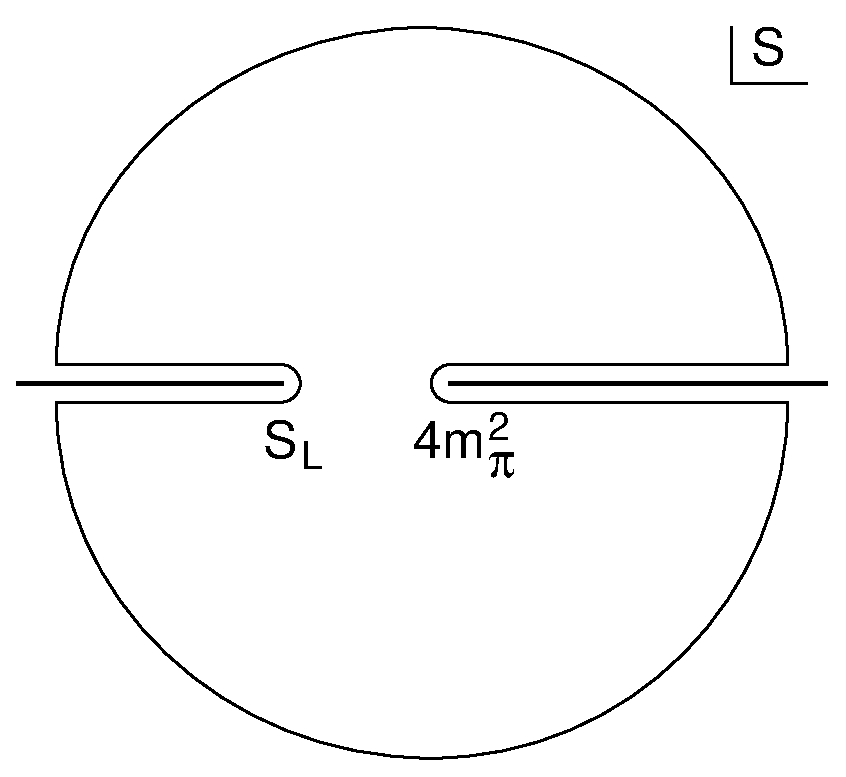
\psfig{file=ijntf1.eps,width=1.5in}} %1.75
\vspace*{8pt}
\caption{A schematic illustration of dissociative recombination. The
direct mechanism, 4m$^2_\pi$ is initiated when the
molecular ion S$_{\rm L}$ captures an electron with 
kinetic energy.\label{fig1}}
\end{figure}

Figures are to be numbered sequentially in Arabic numerals. The
caption must be placed below the figure. Typeset in 8 pt roman with
baselineskip of 10~pt. Use double spacing between a caption and the text
that follows immediately.

Previously published material must be accompanied by written
permission from the author and publisher.

Figures should be referred to in the abbreviated form, 
e.g.~``$\ldots$ in Fig.~\ref{fig1}'' or ``$\ldots$ in   
Figs.~\ref{fig1} and 2''. Where the word ``Figure'' begins a 
sentence, it should be spelled in full.

\section{Tables}

Tables should be inserted in the text as close to the point of
reference as possible. Some space should be left above and below
the table.

Tables should be numbered sequentially in the text in Arabic
numerals. Captions are to be centralized above the tables.  Typeset 
table text and captions in 8 pt roman with baselineskip of 10 pt. 

\begin{table}[ht]
\tbl{Comparison of acoustic for frequencies for piston-cylinder problem.}
{\begin{tabular}{@{}cccc@{}} \toprule
Piston mass & Analytical frequency & TRIA6-$S_1$ model &
\% Error \\
& (Rad/s) & (Rad/s) \\ \colrule
1.0\hphantom{00} & \hphantom{0}281.0 & \hphantom{0}280.81 & 0.07 \\
0.1\hphantom{00} & \hphantom{0}876.0 & \hphantom{0}875.74 & 0.03 \\
0.01\hphantom{0} & 2441.0 & 2441.0\hphantom{0} & 0.0\hphantom{0} \\
0.001 & 4130.0 & 4129.3\hphantom{0} & 0.16\\ \botrule
\end{tabular}}
\end{table}

If tables extend over to a second page, the continuation of
the table should be preceded by a caption, 
e.g.~``Table~2. (Continued)''. 

\section*{Acknowledgments}

This section should come before the References. Dedications and funding
information may also be included here.

\appendix

\section{Appendices}

Use only when absolutely necessary. They
should come before the References. If there is more than one 
appendix, number them alphabetically. Number displayed equations
occurring in the Appendix as follows: (\ref{app1}), (A.2),
etc.
\begin{equation}
\mu(n, t) = {\sum^\infty_{i=1} 1(d_i < t, N(d_i) 
= n)}{\int^t_{\sigma=0} 1(N(\sigma) = n)d\sigma}\,.
\label{app1}
\end{equation}

\section*{References}

References are to be listed in alphabetical order of the author's name
and cited in the text in Arabic numerals within square brackets. 
They can be referred to indirectly, 
e.g.~``$\ldots$ in the statement \cite{2}.'' or used directly,
e.g.~``$\ldots$ see [2] for examples.'' List references using the
style shown in the following examples. For journal names, use the
standard abbreviations.  Typeset references in 9 pt roman.

\begin{thebibliography}{0}

\bibitem{1} A. Alekseev, A. Malkin and E. Meinrenken, Lie group valued
moment maps, {\it J. Differential Geom.} {\bf 48}(3) (1998) 445-495.

\bibitem{2} F. Bouchut, On zero pressure gas dynamics, in 
{\it Advances in Kinetic Theory and Computing}, ed.~B. Perthame, 
Ser. Adv. Math. Appl. Sci., Vol. 22 (World Scientific, 1994),
pp.~171--190.

\bibitem{3} S. K. Godunov and E. Romenskii, {\it Elements of Continuum 
Mechanics and Conservation Laws} (Kluwer Academic/Plenum Publishers,
2003).

\bibitem{4} J. Li and T. Zhang, On the initial-value problem for
zero-pressure gas dynamics, in {\it Proc. 7th Intl. Conf. on Hyperbolic
Problems}, ed. R. Jeltsch (Birkhauser Verlag, 1998), pp.~629--640.

\end{thebibliography}

\end{document}



